\documentclass{article}

% --- Pacchetti utili ---
\usepackage{listings}
\usepackage{xcolor} % Per definire colori personalizzati se vuoi
\usepackage[utf8]{inputenc} % Codifica del testo
\usepackage[italian]{babel}   % Lingua italiana
\usepackage{amsmath}        % Per equazioni matematiche (se necessarie)
\usepackage{graphicx}       % Per includere immagini (se necessarie)
\usepackage{geometry}       % Per gestire i margini della pagina
\geometry{a4paper, total={16cm,24cm}, left=2.5cm, top=2.5cm} % Esempio di impostazione margini

% --- Configurazione per VHDL con listings ---
\lstset{
    language=VHDL,                % Specifica il linguaggio come VHDL
    basicstyle=\ttfamily\small,   % Stile del testo: font monospaced e dimensione piccola
    numbers=left,                 % Numera le righe a sinistra
    numberstyle=\tiny\color{gray}, % Stile dei numeri di riga
    frame=single,                 % Aggiunge una cornice attorno al blocco di codice
    framesep=5pt,                 % Spazio tra cornice e codice
    framerule=0.5pt,              % Spessore della cornice
    rulecolor=\color{black},      % Colore della cornice
    showstringspaces=false,       % Non mostrare spazi nelle stringhe
    tabsize=2,                    % Dimensione del tab
    breaklines=true,              % Permette di spezzare righe lunghe
    captionpos=b,                 % Posizione della didascalia (b=bottom, t=top)
    keywordstyle=\color{blue}\bfseries, % Colore e stile per le parole chiave
    identifierstyle=\color{black},      % Stile per gli identificatori
    commentstyle=\color{green!50!black}, % Colore per i commenti
    stringstyle=\color{orange!70!black}, % Colore per le stringhe
    literate={_}{{\_}}1,          % Permette l'underscore nel codice VHDL
    morekeywords={entity, is, port, end, architecture, behavioral, signal, std_logic, std_logic_vector, in, out, process, begin, if, else, elsif, then, end, loop, variable, to_signed , constant, resize} % Aggiungi altre parole chiave VHDL se necessario
}

% --- Personalizzazione della pagina del titolo ---
% Ridefiniamo il comando \maketitle per avere più controllo sullo stile
\makeatletter
\renewcommand{\maketitle}{%
  \begin{titlepage}%
    \centering%
    \vspace*{2cm}% Spazio dall'alto della pagina
    {\fontsize{28}{30}\selectfont \bfseries \@title \par}% Titolo più grande e in grassetto
    \vspace{1.5cm}% Spazio tra titolo e autore
    {\fontsize{18}{20}\selectfont \@author \par}% Autore più grande
    \vspace{1cm}% Spazio tra autore e data
    {\fontsize{14}{16}\selectfont \@date \par}% Data più grande
    \vfill% Riempie lo spazio rimanente per centrare verticalmente
    % Puoi aggiungere qui un logo o altre informazioni se necessario
    \vspace*{2cm}% Spazio dal basso della pagina
  \end{titlepage}%
}
\makeatother

% --- Informazioni del documento ---
\title{\Huge Prova Finale di Reti Logiche \\ \Large Anno 2024/2025}
\author{Alberto Pini e Davide Redaelli\\(212524 - 215263)}
\date{\today} % O puoi specificare una data fissa, es: \date{5 Luglio 2025}

\begin{document}

% --- Pagina del titolo ---
\maketitle
\thispagestyle{empty} % Non mostra il numero di pagina sulla pagina del titolo

\newpage % Forza una nuova pagina

% --- Sommario ---
\tableofcontents
\thispagestyle{plain} % Mostra il numero di pagina sul sommario

\newpage % Forza una nuova pagina

% --- Contenuto della relazione ---






\section{Introduzione}

In questo progetto di Reti Logiche ci è stato chiesto di sviluppare un programma in VHDL che sia in grado di programmare un FPGA. 

\section{Analisi Specifica}
L'FPGA da programmare lavora con una memoria costituita da metadati iniziali e una sequenza di $K$ parole, ciascuna referenziata con $W_i$. Il Chip dovrà "iterare" la memoria mentre calcola e scrive i risultati.

\subsection{Interfaccia del Componente}

Diagramma delle porte

\begin{figure}[h!]
    \centering
    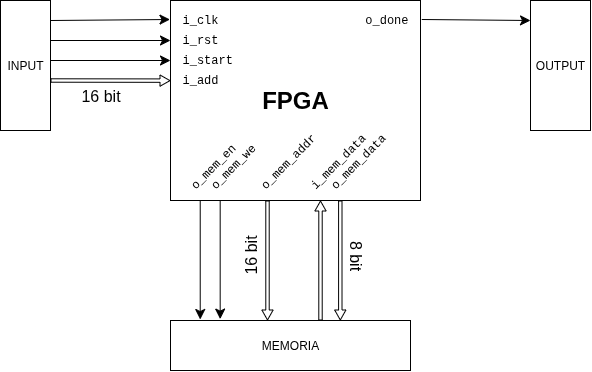
\includegraphics[width=0.8\textwidth]{resources/fpga.png} % Sostituisci con il nome della tua immagine
    \caption{Diagramma delle porte}
    \label{fig:png}
\end{figure}
\noindent Notare che nel contesto di development sia \texttt{INPUT} che \texttt{OUTPUT} che \texttt{MEMORIA} fanno tutti parte di un unico chip non sintetizzabile che corrisponde al Testbench.

\begin{figure}[h!]
    \centering
    \begin{lstlisting}[caption=In \texttt{VHDL} l'entità componente viene definita in questo modo, label=lst:entity_vhdl]
entity project_reti_logiche is
    port (
        i_clk      : in std_logic;
        i_rst      : in std_logic;
        i_start    : in std_logic;
        i_add      : in std_logic_vector(15 downto 0);
        o_done     : out std_logic;
        o_mem_addr : out std_logic_vector(15 downto 0);
        i_mem_data : in std_logic_vector(7 downto 0);
        o_mem_data : out std_logic_vector(7 downto 0);
        o_mem_we   : out std_logic;
        o_mem_en   : out std_logic
    );
end project_reti_logiche;
    \end{lstlisting}
\end{figure}

\noindent Descrizione delle porte del componente:

\begin{itemize}
    \item \texttt{i\_clk} clock di sistema
    \item \texttt{i\_rst} segnale di reset asincrono
    \item \texttt{i\_start} segnale che indica la fine della scrittura in memoria degli input da parte del testbench e, conseguentemente, la possibilità di iniziare il calcolo da parte del chip
    \item \texttt{i\_add} $[15-0]$ address della memoria da cui leggere il primo bit
    \item \texttt{o\_done} segnale da alzare una volta che si è finito di scrivere l'ultimo risultato
\end{itemize}

Le altre porte sono per la lettura e scrittura della memoria

\begin{itemize}
    \item \texttt{o\_mem\_en} segnale per attivare la memoria in lettura e potenzialmente anche in lettura
    \item \texttt{o\_mem\_we} segnale per attivare la modalità di lettura della memoria
    \item \texttt{o\_mem\_addr} $[15-0]$ address della memoria su cui il chip vuole lavorare (sia in lettura che scrittura)
    \item \texttt{i\_mem\_data} $[7-0]$ segnale fornito dal chip alla memoria per memorizzare il valore in \texttt{o\_mem\_addr} (con $\texttt{o\_mem\_we} = \texttt{o\_mem\_en} = 1$)
    \item \texttt{o\_mem\_data} $[7-0]$ segnale fornito al chip dalla memoria corrispondente al valore risultante della precedente lettura (con $\texttt{o\_mem\_we} = 0$ e $\texttt{o\_mem\_en} = 1$)
\end{itemize}

Queste porte sono meglio approfondite nella sezione dedicata \ref{subsubsec:memoria}.

\subsection{Struttura Memoria}

Tutti i dati da utilizzare sono memorizzati sequenzialmente a partire da un indirizzo specificato
(ADD). I dati iniziali comprendono:
\begin{itemize}
    \item \textbf{17 byte} che indicano la lunghezza della sequenza, l'ordine del filtro differenziale e i coefficienti.
    \begin{itemize}
        \item \textbf{K1} e \textbf{K2}: due byte che indicano la lunghezza della sequenza K dei dati di W (\texttt{K1} è il byte più significativo, lunghezza minima = 7 byte).
        \item \textbf{S}: un byte che indica quale filtro selezionare tra ordine 3 e ordine 5 (bit meno significativo: 0 $\rightarrow$ ordine 3, 1 $\rightarrow$ ordine 5).
        \item Da \textbf{C1} a \textbf{C14}: $14$ byte contenenti i coefficienti dei filtri. I coefficienti sono presenti per entrambi i filtri indipendentemente dal valore di \texttt{S}. Per esempio
        \begin{itemize}
            \item Ordine 3: c=[\texttt{0, -1, 8, 0, -8, 1, 0}] da \texttt{C1} a \texttt{C7}, normalizzazione $n=12$.
            \item Ordine 5: c=[\texttt{1, -9, 45, 0, -45, 9, -1}] da \texttt{C8} a \texttt{C14}, normalizzazione $n=60$.
        \end{itemize}
    \end{itemize}
    \item \textbf{K byte} da elaborare, contenenti valori tra -128 e +127, che rappresentano il vettore numerico
    da processare.
\end{itemize}

Graficamente:
\begin{figure}[h!]
    \centering
    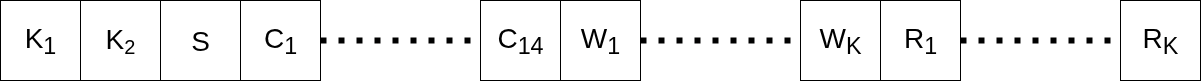
\includegraphics[width=0.8\textwidth]{resources/memoria.png}
    \caption{Struttura della memoria}
    \label{fig:png}
\end{figure}

\noindent Quindi unendo gli $8$ bit di $K_1$ con gli altri $8$ bit di $K_2$ ottengo un numero $K$ di $16$ bit. Questo numero è fondamentale per:
\begin{itemize}
    \item capire quando terminare la lettura delle $W_i$ da processare (quando si arriva a $17 + K$ byte)
    \item saper in che indirizzo di memoria scrivere il primo risultato $R_1$ (al $(17+K+1)$esimo byte)
\end{itemize}

\subsection{Computare il Risultato}

Il filtro applicato ha la seguente formula matematica:
$$
f'(i) = \frac{1}{n} \sum_{j=-I}^{I} C_j \cdot f[j+i]
$$
Dove \textbf{I=2} per il filtro di ordine 3 e \textbf{I=3} per il filtro di ordine 5.

\noindent Bisogna inoltre assicurarsi che il risultato del filtraggio prima della normalizzazione ($\sum C_j \cdot f[j+i]$) abbia un numero di bit adeguato per la sua rappresentazione.

\noindent La divisione per \texttt{n} viene approssimata come segue:
\begin{itemize}
    \item $\frac{1}{12} \approx \frac{1}{16} + \frac{1}{64} + \frac{1}{256} + \frac{1}{1024}$
    \item $\frac{1}{60} \approx \frac{1}{64} + \frac{1}{1024}$
\end{itemize}

Poiché ogni shift a destra equivale a una divisione per due, nel caso di numeri negativi si applica
una correzione: se $\text{val} \gg m < 0$ , si aggiunge $+1$ per ridurre l'errore di troncamento.

Per esempio:
\begin{gather*}
-40 \times \frac{1}{12} \approx (-40 \gg 4 + 1) + (-40 \gg 6 + 1) + (-40 \gg 8 + 1) + (-40 \gg 10 + 1)
\end{gather*}

\subsection{Funzionamento Modulo}

Il modulo ha i seguenti segnali:
\begin{itemize}
    \item Ingressi:
    \begin{itemize}
        \item \texttt{i\_start} = \textbf{START} (1 bit): avvia l'elaborazione.
        \item \texttt{i\_add} (16 bit): indirizzo della memoria di partenza.
        \item \texttt{i\_clk} = \textbf{CLOCK}
        \item \texttt{i\_rst} = \textbf{RESET}.
    \end{itemize}
    \item Uscite:
    \begin{itemize}
        \item \texttt{o\_done} = \textbf{DONE} (1 bit): indica la fine dell'elaborazione al testbench.
    \end{itemize}
\end{itemize}

\noindent Il modulo segue la seguente sequenza operativa:
\begin{enumerate}
    \item All'avvio \texttt{RESET=1} e \texttt{DONE=0}.
    \item Quando \texttt{RESET} torna a \texttt{0}, il modulo attende che, quando il \texttt{CLOCK} sale ad $1$, \texttt{START} sia pari a $1$.
    \item Legge i dati da memoria, esegue il filtraggio e scrive i risultati.
    \item Alla fine dell'elaborazione, alza \texttt{DONE=1} per segnalare al testbench che il moduolo ha finito il suo lavoro.
    \item Il modulo attende che \texttt{START} torni a \texttt{0} prima di una nuova fase di computazione.
    \item Infine il modulo setta \texttt{DONE=0} per segnalare al testbench che è pronto a ricevere un nuovo \texttt{START=1}.
\end{enumerate}

In qualsiasi momento \texttt{RESET} può passare da $0 \to 1$ e, in modo asincrono (quindi indipendentemente dal segnale \texttt{i\_clk}), il componente deve essere in grado di:
\begin{enumerate}
    \item fermare l'esecuzione
    \item ...
\end{enumerate}

\subsection{Lavorare con la Memoria}\label{subsubsec:memoria}

La comunicazione con la memoria esterna, gestita a livello del Top Module, avviene tramite un'interfaccia standardizzata che include i seguenti connettori:
\begin{itemize}
    
    \item \texttt{o\_mem\_en} (Output, \texttt{std\_logic}): Questo segnale viene asserito a $1$ per abilitare la comunicazione con la memoria esterna, sia per operazioni di lettura che di scrittura. Quando \texttt{o\_mem\_en} è $0$, la memoria è disabilitata e non risponde alle richieste.
    
    \item \texttt{o\_mem\_we} (Output, \texttt{std\_logic}): Questo segnale definisce il tipo di operazione sulla memoria. Se \texttt{o\_mem\_we} è $0$, l'operazione è di lettura. Se \texttt{o\_mem\_we} è $1$, l'operazione è di scrittura. È fondamentale che \texttt{o\_mem\_en} sia attivo quando \texttt{o\_mem\_we} viene pilotato.
    
    \item \texttt{o\_mem\_addr} (Output, \texttt{std\_logic\_vector(15 downto 0)}): Questo è l'indirizzo a 16 bit nella memoria su cui il sistema desidera operare. Viene utilizzato sia per le letture che per le scritture, specificando l'indirizzo di memoria target (in cui scrivere o da cui leggere).
    
    \item \texttt{o\_mem\_data} (Output, \texttt{std\_logic\_vector(7 downto 0)}): Questa porta serve ad "inviare" il dato a 8 bit che il componente intende scrivere nella memoria. Questo segnale è valido e viene letto dalla memoria solo quando \texttt{o\_mem\_en=1} e \texttt{o\_mem\_we = 1}.
    
    \item \texttt{i\_mem\_data} (Input, \texttt{std\_logic\_vector(7 downto 0)}): Questo connettore riceve il dato a 8 bit letto dalla memoria esterna. Il valore su \texttt{i\_mem\_data} è valido e deve essere campionato dal componente quando \texttt{o\_mem\_en=1} e \texttt{o\_mem\_we=0}, e dopo il tempo di propagazione della memoria.
\end{itemize}

\noindent Data la mancanza di un segnale di acknowledgment da parte della memoria, consideriamo l'operazione conclusa sempre $1$ ciclo di clock dopo aver mandato il comando.


\subsubsection{Operazione di Scrittura:}
\begin{enumerate}
    
    \item Al fronte di salita del clock $T_0$, il sistema asserisce \texttt{o\_mem\_en = 1}, \texttt{o\_mem\_we = 1}, \texttt{o\_mem\_addr} all'indirizzo desiderato e \texttt{o\_mem\_data} con il valore da scrivere.
    
    \item Al fronte di salita del clock $T_1$ (cioè 1 CLK dopo), la scrittura nella memoria è considerata completata e il dato è stato memorizzato all'indirizzo specificato. Il sistema può quindi modificare i due segnali di controllo oppure avviare una nuova operazione.
\end{enumerate}

\subsubsection{Operazione di Lettura:}
\begin{enumerate}
    \item Al fronte di salita del clock $T_0$, il sistema asserisce \texttt{o\_mem\_en = 1}, \texttt{o\_mem\_we = 0} e \texttt{o\_mem\_addr} all'indirizzo da leggere.
    \item Al fronte di salita del clock $T_1$ (cioè 1 CLK dopo), il dato letto dalla memoria sarà disponibile e stabile sul connettore \texttt{i\_mem\_data} e potrà essere campionato dal sistema. Il sistema può quindi disasserire i segnali di controllo o avviare una nuova operazione.
\end{enumerate}

\subsection{Esempio}

\begin{figure}[h!]
    \centering
    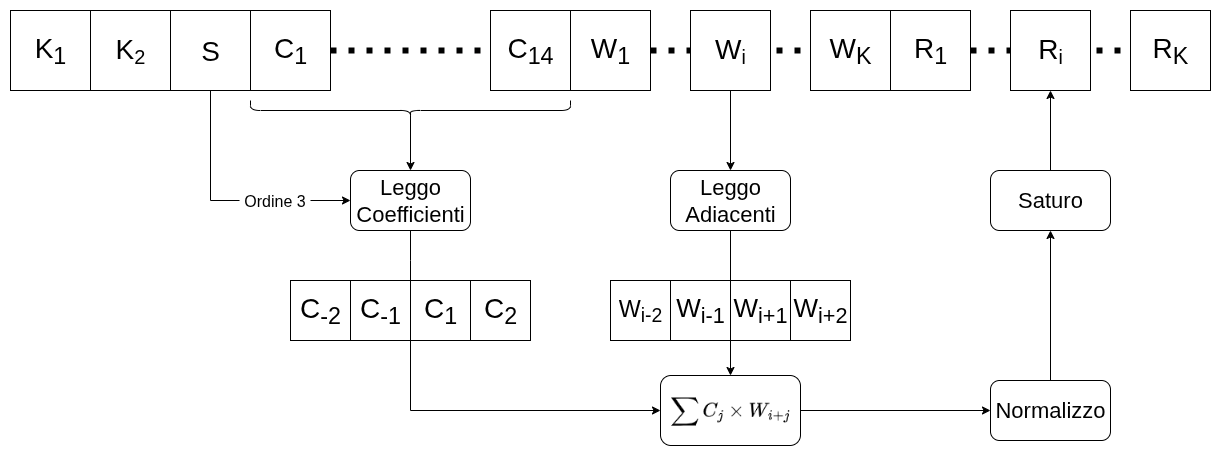
\includegraphics[width=0.8\textwidth]{resources/esempio.png}
    \caption{Diagramma di esempio}
    \label{fig:png}
\end{figure}

Per illustrare il processo di filtraggio differenziale, consideriamo l'applicazione di un filtro di ordine 3 a una sequenza generica di dati. Si assume che il modulo abbia già letto dalla memoria i parametri iniziali, ovvero la lunghezza della sequenza $K$, il bit di selezione del filtro $S$ (che indica l'uso di un filtro di ordine 3), e i coefficienti del filtro. La sequenza dei coefficienti sarà composta da $C_{-3}, C_{-2}, C_{-1}, C_1, C_2 C_3$ (letti in base all'ordine del filtro) e il valore di normalizzazione $n$. L'indirizzo di inizio dei dati in input è $\text{ADD}_W$, e l'indirizzo dove verranno scritti i risultati è $\text{ADD}_R$.

Il processo iterativo per il calcolo di ciascun valore filtrato $R_i$ è il seguente:
\begin{enumerate}
    \item \textbf{Lettura dei dati di input:} Per calcolare il valore $R_i$, il modulo deve accedere ai valori $W$ circostanti la posizione $i$ nella memoria. Nello specifico, per un filtro di ordine 3, saranno necessari i valori $W_{i-2}, W_{i-1}, W_{i+1}, W_{i+2}$ ($W_i$ non è necessario dato che si assume che $C_0=0$). Questi vengono letti dagli indirizzi di memoria appropriati, che sono $ADD_W + (i-2)$, $ADD_W + (i-1)$, $ADD_W + (i+1)$, $ADD_W + (i+2)$. Si noti che per i valori all'inizio o alla fine della sequenza $W$ (cioè quando gli indici $i-2$, $i-1$, $i+1$, $i+2$ eccedono i limiti della sequenza valida), i valori corrispondenti a $W$ non esistenti sono considerati pari a $0$.
    
    \item \textbf{Calcolo della somma pesata:} Viene calcolata la somma pesata dei valori di input con i rispettivi coefficienti del filtro. La formula generale per un filtro differenziale è 
    $$R_i^\text{raw} = \sum_{j=-l}^{+l} C_j \times W_{i+j}\ \ \, \text{dove}\ l= \left\{ \begin{array}{cl} 2 \text{ per il filtro di ordine 3} \\ 3 \text{ per il filtro di ordine 5} \end{array} \right.$$
    Pertanto, il valore intermedio (di ordine $3$) sarà:
    $$R_i^\text{raw} = (C_{-2} \times W_{i-2}) + (C_{-1} \times W_{i-1}) + (C_1 \times W_{i+1}) + (C_2 \times W_{i+2})$$
    Si assume che i coefficienti $C_j$ siano quelli specificati per il filtro di ordine 3, come ad esempio i coefficienti non nulli $C_{-2}, C_{-1}, C_1, C_2$ dalla specifica $c=[-1, 8, -8, 1]$. Se invece stessimo filtrando in ordine $5$ i $C_j$ sarebbero stati $6$ in totale ($C_{-3}, C_{-2}, C_{-1}, C_1, C_2 C_3$).
    
    \item \textbf{Normalizzazione:} Il valore $R_i^\text{raw}$ ottenuto deve essere normalizzato dividendolo per il coefficiente $n$. Questa divisione è approssimata come una somma di shift a destra (divisioni per potenze di 2). Per il filtro di ordine 3, $n=12$, approssimato come $1/16+1/64+1/256+1/1024$. Per minimizzare l'errore di troncamento per i numeri negativi, viene aggiunto $1$ al risultato di un singolo shift se il valore shiftato è negativo.
    \item \textbf{Saturazione:} Dopo la normalizzazione, il valore $R_i$ risultante viene confrontato con l'intervallo valido di $[-128, +127]$. Se $R_i$ è inferiore a $-128$, viene saturato a $-128$. Se $R_i$ è superiore a $+127$, viene saturato a $+127$.
    \item \textbf{Scrittura in memoria:} Il valore finale $R_i$ viene scritto in memoria all'indirizzo $\text{ADD}_R + i$.
\end{enumerate}
Questo ciclo si ripete per tutti i $K$ valori della sequenza, dopodiché il modulo segnala il completamento dell'operazione.

\section{Architettura del Componente}

Per questo progetto abbiamo creato un unico modulo (\texttt{project\_reti\_logiche}) che agisce ovviamente da \texttt{top\_module}. Al suo interno è presente un unico processo contenente tutta la logica dell'FPGA...

\subsection{FSM e Descrizione Stati }
Ogni transizione da uno stato ad un altro nella macchina a stati finiti, include una transizione intermedia ad uno stato di "attesa", necessario per permettere ai testbench di interagire con la memoria e di inviare al successivo ciclo di clock i corretti segnali richiesti dal modulo.

Prima della transizione allo stato WAITING, sarà computato e modificato il segnale \texttt{next\_state}, che rappresenta dunque il prossimo stato. 
 Figura \ref{fig:png}

\noindent Inoltre il segnale \texttt{i\_rst} agisce come segnale asincrono. Ciò vuol dire che, indipendentemente dal segnale di clock, l'attivazione di \texttt{i\_rst} porta a:
\begin{itemize}
    \item reset di ogni segnale interno 
    \item settaggio di \texttt{state <= WAITING} e di \texttt{next\_state <= START} 
\end{itemize}

Di seguito i diagrammi del cambio di stato \ref{WAITING_STATE_FSM} e della FSM principale \ref{mainFSM}.

\newpage
\begin{figure}[h!]
    \centering
    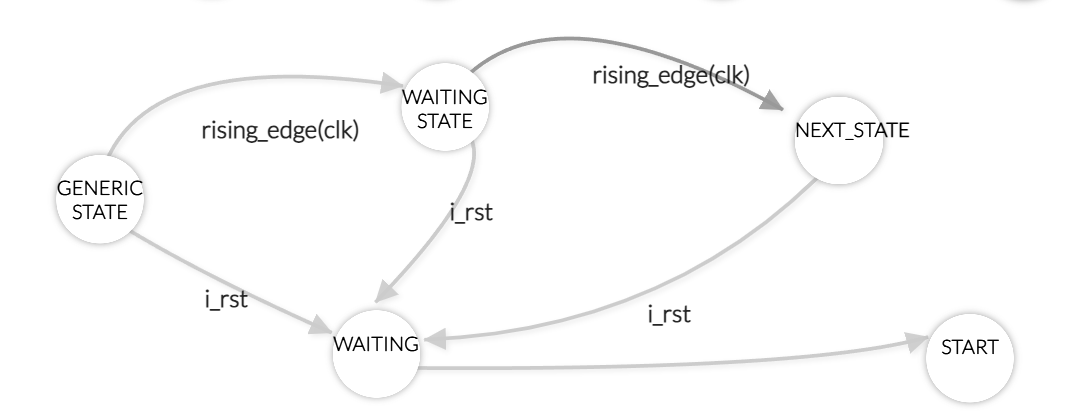
\includegraphics[width=0.8\textwidth]{resources/basicSchema.png}
    \caption{Generico cambio di stato con segnale di reset}
    \label{WAITING_STATE_FSM}
\end{figure}

\begin{figure}[h!]
    \centering
    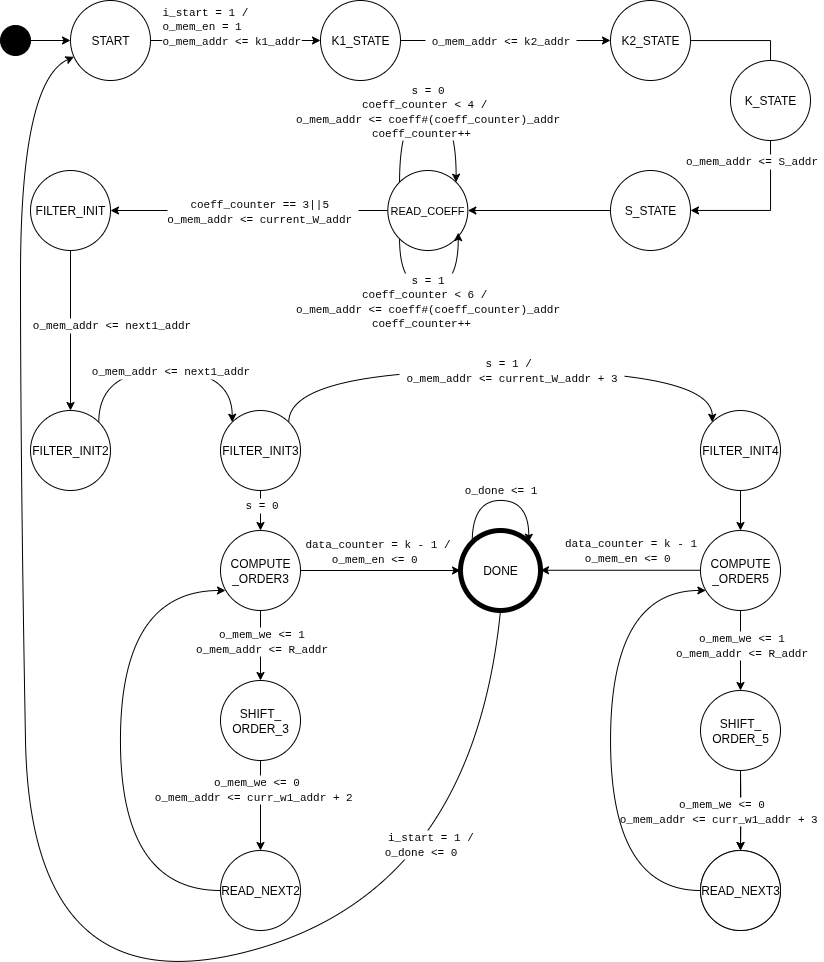
\includegraphics[width=0.8\textwidth]{resources/mainFSM.png}
    \caption{Diagramma generale FMS}
    \label{mainFSM}
\end{figure}

\subsection{Segnali e Variabili}

Questi segnali sono utilizzati per la gestione interna dei dati e il controllo del flusso all'interno del modulo:
\begin{itemize}
    \item \textbf{Segnali per gli stati}:
    \begin{itemize}
        \item \texttt{next\_state}: Segnale di tipo \texttt{state\_type} (stati descritti precedentemente) che memorizza lo stato futuro a cui la FSM transirà nel prossimo ciclo di clock.
        \item \texttt{state}: Segnale di tipo \texttt{state\_type} che rappresenta lo stato corrente in cui si trova la FSM.
    \end{itemize} 
    
    \item \textbf{Contatori interni}: 
    \begin{itemize}
        \item \texttt{data\_counter}: Contatore intero che tiene traccia del numero di parole $W$ elaborate e funge da indice per l'accesso ai dati in input e la scrittura dei risultati in output.
        \item \texttt{coeff\_counter}: Contatore intero che tiene traccia del numero di coefficienti del filtro letti durante la fase di inizializzazione.
    \end{itemize}

    \item \textbf{Segnali per memorizzare i coefficienti}: 
    \begin{itemize}
        \item \texttt{c\_n2\_3}, \texttt{c\_n1\_3}, \texttt{c\_p1\_3}, \texttt{c\_p2\_3}: Segnali a 8 bit (\texttt{signed}) che memorizzano i coefficienti specifici per il filtro di ordine 3. Corrispondono ai coefficienti $C_{-2}, C_{-1}, C_{+1}, C_{+2}$ dalla specifica, assumendo $C_0$ sia un valore centrale e altri coefficienti siano impliciti o zero.
        \item \texttt{c\_n3\_5}, \texttt{c\_n2\_5}, \texttt{c\_n1\_5}, \texttt{c\_p1\_5}, \texttt{c\_p2\_5}, \texttt{c\_p3\_5}: Segnali a 8 bit (\texttt{signed}) idem a prima ma per il filtro di ordine 5.
    \end{itemize}

    \item \textbf{Segnali della "sliding window"}:
    \begin{itemize}
        \item \texttt{prev3}, \texttt{prev2}, \texttt{prev1}: Segnali a 8 bit (\texttt{signed}) che contengono i valori di input $W$ precedenti all'attuale valore \texttt{current\_W} nel buffer di scorrimento.
        \item \texttt{current\_W}: Segnale a 8 bit (\texttt{signed}) che contiene il valore di input $W$ attualmente in elaborazione.
        \item \texttt{next1}, \texttt{next2}, \texttt{next3}: Segnali a 8 bit (\texttt{signed}) che contengono i valori di input $W$ successivi all'attuale valore \texttt{current\_W} nel buffer di scorrimento.
    \end{itemize}
    Questi valori alla fine di ogni calcolo vengono shiftati per far spazio al nuovo valore letto in \texttt{next2} o \texttt{next3} a seconda dell'ordine del filtro.

    \item \textbf{Altri segnali interni}:
    \begin{itemize}
        \item \texttt{mem\_w1\_addr}: Indirizzo a 16 bit che punta all'inizio della sequenza di dati $W$ da filtrare in memoria. È calcolato sommando l'indirizzo base \texttt{i\_add} e l'offset dei metadati iniziali (ovvero 17 = 3 byte per $K$ e $S$ + 14 byte per i coefficienti).
        \item \texttt{mem\_init\_addr}: Indirizzo a 16 bit che memorizza l'indirizzo di partenza \texttt{i\_add} fornito all'inizio dell'esecuzione, usato come base per accedere ai metadati.
        \item \texttt{k1}, \texttt{k2}: Segnali a 8 bit che memorizzano i due byte letti dalla memoria che insieme formano la lunghezza $K$ della sequenza di input.
        \item \texttt{k}: Segnale a 16 bit (\texttt{unsigned}) che memorizza la lunghezza effettiva della sequenza di dati $W$ da elaborare.
        \item \texttt{s}: Segnale a 1 bit (\texttt{std\_logic}) che indica il tipo di filtro: \texttt{0} per l'ordine 3, \texttt{1} per l'ordine 5.
    \end{itemize}
    
\end{itemize}


\noindent Ci sono poi le variabili che vengono utilizzate temporaneamente all'interno del processo sequenziale per calcoli intermedi e non mantengono il loro valore tra un ciclo di clock e l'altro:
\begin{itemize}
    \item \texttt{tmp\_k}: Variabile a 16 bit (\texttt{std\_logic\_vector}) utilizzata per concatenare \texttt{k1} e \texttt{k2} prima di assegnare il risultato a \texttt{k}.
    \item \texttt{tmp\_s}: Variabile a 1 bit (\texttt{std\_logic}) utilizzata per una copia temporanea del bit di selezione del filtro \texttt{s} per il controllo immediato del flusso.
    \item \texttt{tmp\_p3}, \texttt{tmp\_p2}, \texttt{tmp\_p1}, \texttt{tmp\_n1}, \texttt{tmp\_n2}, \texttt{tmp\_n3}: Variabili a 32 bit (\texttt{signed}) utilizzate per memorizzare i prodotti intermedi dei coefficienti per i valori di input. Vengono utilizzate con una larghezza maggiore per prevenire overflow durante le moltiplicazioni.
    \item \texttt{tmp\_sum}: Variabile a 32 bit (\texttt{signed}) che accumula la somma totale dei prodotti parziali dei coefficienti e dei valori di input.
    \item \texttt{tmp\_res}: Variabile a 32 bit (\texttt{signed}) che contiene il risultato del filtraggio dopo la normalizzazione, prima dell'applicazione della saturazione e della conversione a 8 bit.
\end{itemize}
In particolare vengono utilizzate in questo modo nello stato di \texttt{COMPUTE\_ORDER\_3}

\begin{figure}[h!]
    \centering
    \begin{lstlisting}[caption=Calcolo mediante variabili temporanee]
tmp_n2 := resize(c_n2_3, 16) * resize(prev2, 16);
tmp_n1 := resize(c_n1_3, 16) * resize(prev1, 16);
tmp_p1 := resize(c_p1_3, 16) * resize(next1, 16);
tmp_p2 := resize(c_p2_3, 16) * resize(next2, 16);

tmp_sum := tmp_n2 + tmp_n1 + tmp_p1 + tmp_p2;
tmp_res := shift_right (tmp_sum, 4) + shift_right (tmp_sum, 6) 
         + shift_right (tmp_sum, 8) + shift_right (tmp_sum, 10);
if tmp_sum < to_signed(0, 32) then
   tmp_res := tmp_res + 4;
end if;
    \end{lstlisting}
\end{figure}




\section{Risultati Sperimentali}

\subsection{Introduzione}
Il modulo è stato sottoposto ai seguenti TestBench, superandoli tutti fino alla fase di simulazione post sintesi functional.
Per il testbench 2345 è stata effettuata anche la 

tabella TB ...

I testbench a cui si fa riferimento nella tabella sono contenuti nella directory \texttt{TestBenches} nella cartella root della repo.

\subsection{Sintesi}
risultati della sintesi... con screen shot

\subsection{Post-Sintesi}

\subsection{TestBench}

\subsubsection{Risultati TB standard}

\subsubsection{TB custom per edge cases...}

\section{Conclusioni}


link alla repo...

\end{document}